\section{Aufgabe 10}
Gegeben ist die Population $P_0$ mit den Werten:
\begin{align}
  &\mu_x = 0 \\
  &\mu_y = 3 \\
  &\sigma_x = 3{,}5 \\
  &\sigma_y = 2{,}6 \\
  &\rho=0,9.
\end{align}
Ebenso ist eine Population $P_1$ gegeben. Bei dieser sind die Werte in $x$ gegeben durch:
\begin{align}
  &\mu_x = 6 \\
  &\sigma_x = 3{,}5 \text{.}
\end{align}
Für die Werte in y sind folgende Zusammenhänge gegeben:
\begin{align}
  &\text{E}(y\lvert x) = \mu_{y\lvert x} = a + bx \text{ mit } a  = -0{,}5 \text{  und } b=0{,}6 \label{eqn:Exy0} \\
  &\text{Var}(y\lvert x) = \sigma_{y\lvert x}^2 = 1
\end{align}


\subsection{Teilaufgabe a)}
\subsubsection{Zeigen der 2D-Gaußverteilung}
Die Formel für die bedingte Wahrscheinlichkeit der bivariaten Normalverteilung lautet:
\begin{equation}
f(y\lvert x) = \frac{1}{\sqrt{2\pi} \sigma_y \sqrt{1-\rho^2}} \cdot \,
\exp\left(-\frac{1}{2(1-\rho^2)} \left [ \frac{\tilde{y}}{\sigma_y}-\rho\frac{\tilde{x}}{\sigma_x} \right]^2 \right) \text{.}
\end{equation}
\begin{center}
  \small {wobei \text{$\tilde{x} = x - \mu_x$ und $\tilde{y} = y - \mu_y$}}
\end{center}
Für die Wahrscheinlichkeitsdichtefunktion einer bivariaten Normalverteilung gilt dagegen:
\begin{equation}
f(x,y) =
      \frac{1}{2 \pi  \sigma_x \sigma_y \sqrt{1-\rho^2}}
      \exp\left(
        -\frac{1}{2(1-\rho^2)}\left[
          \frac{(x-\mu_x)^2}{\sigma_x^2} +
          \frac{(y-\mu_y)^2}{\sigma_y^2} -
          \frac{2\rho(x-\mu_x)(y-\mu_y)}{\sigma_x \sigma_y}
        \right]
      \right)\,, \label{eqn:f(xy)}
\end{equation}
Mit $f(x,y) = g(x) f(y \lvert x)$ folgt mit
\begin{equation}
g(x) = \frac{\sqrt{2(1-\rho^2)}}{2 \pi  \sigma_x \sigma_y \sqrt{1-\rho^2}} \sqrt{\pi} \sigma_y \cdot \,
       \exp\left( -\frac{1}{2} \left(\frac{x-\mu_x}{\sigma_x}\right)^2\right)
\end{equation}
der Zusammenhang
\begin{equation}
f(x,y) = \frac{1}{2 \pi  \sigma_x \sigma_y \sqrt{1-\rho^2}} \cdot \,
         \exp\left(-\frac{1}{2} \left(\frac{x-\mu_x}{\sigma_x}\right)^2
         - \frac{1}{2(1-\rho^2)} \left(\frac{y-\mu_y}{\sigma_y}-\rho\frac{x-\mu_x}{\sigma_x} \right)^2\right)\,.
\end{equation}
Durch Umformungen erhält man die Gleichung \eqref{eqn:f(xy)}, da:
\begin{equation}
  -\frac{(x-\mu_x)^2}{\sigma_x^2} \frac{\rho^2}{2(1-\rho^2)} - \frac{(x-\mu_x)^2}{2\sigma_x^2} = - \frac{(x-\mu_x)^2}{\sigma_x^2} \frac{1}{2(1-\rho^2)}
\end{equation}

\subsubsection{Bestimmen der Werte}
Für die Berechnung der Werte werden folgende Gleichungen genutzt:
\begin{align}
  \sigma_{y\lvert x}^2 = (1-\rho^2)\sigma_y^2 \label{eqn:sig}\\
  \text{E}(y\lvert x) = \rho \frac{\sigma_y}{\sigma_x} (x-\mu_x) + \mu_y \label{eqn:Exy} \\
\end{align}
Bei einem Koeffizientenvergleich der Gleichung \eqref{eqn:Exy} mit \eqref{eqn:Exy0} ergeben sich folgende Zusammenhänge:
\begin{align}
  b  &= \frac{\sigma_y}{\sigma_x} \cdot \rho \label{eqn:b} \\
a &= - \rho \frac{\sigma_y}{\sigma_x} \mu_x + \mu_y
\end{align}
Aus \eqref{eqn:b} und \eqref{eqn:sig} ergibt sich der Zusammenhang
\begin{equation}
  p=\sqrt{\frac{1}{1+\frac{\sigma^2_{y\lvert x}}{b^2 \sigma^2_x}}} \approx 0,75
\end{equation}
womit sich $\sigma_y=\sqrt{\frac{\sigma_{y\lvert x}}{1-p^2}} \approx 1,51$ und $\mu_y=\alpha+\frac{\rho \mu_x}{\sigma_x} \cdot \frac{\sigma_{y\lvert x}}{\sqrt{1-p^2}} \approx 1,44 $ ergeben .


\subsection{Teilaufgabe b)}
Es ergibt sich folgender Scatter-Plot:
\begin{figure}[H]
  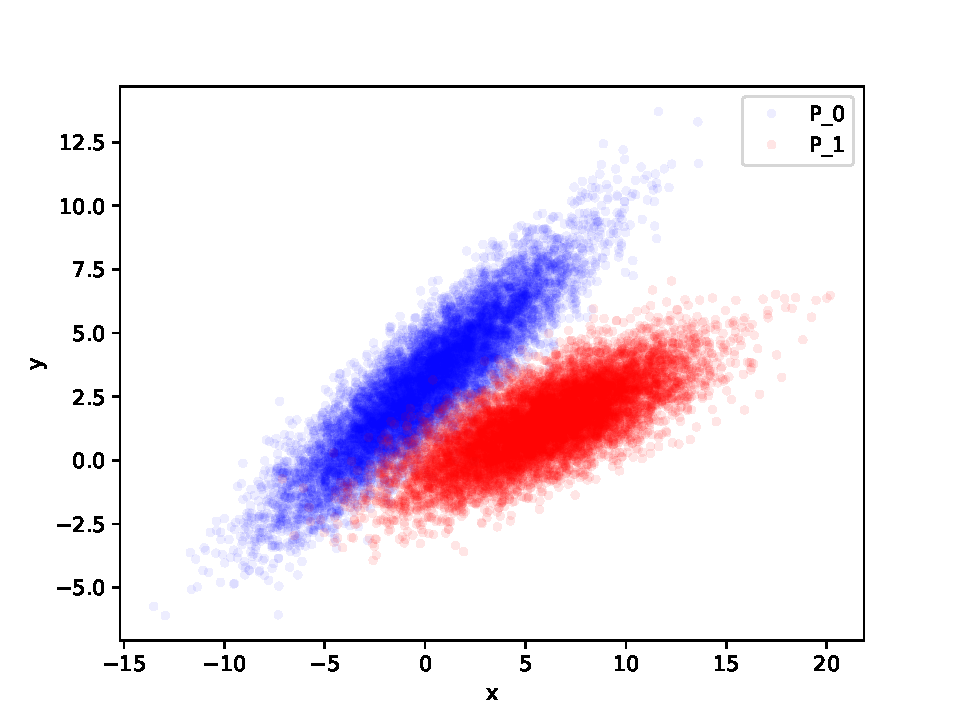
\includegraphics{Aufgabe10/Populationen.pdf}
  \caption{Scatter-Plot}
  \label{}
\end{figure}

\subsection{Teilaufgabe c)}
es ergeben sich folgende Ergebnisse:
\begin{console1}{Population 0}
  Mittelwerte von P0:  [0.00781587 3.00831114] \\
  Varianz von x0:  12.14051138946726 \\
  Varianz von y0:  6.654329986905046 \\
  Kovarianz cov(x, y):  8.095175577329087 \\
  Korrelation rho:  0.9006490919236851
\end{console1}

\begin{console1}{Population 1}
  Mittelwerte von P0:  [6.00106294 1.41078796] \\
  Varianz von x0:  12.258004437206726 \\
  Varianz von y0:  2.2870875071918366 \\
  Kovarianz cov(x, y):  3.9966098123833347 \\
  Korrelation rho:  0.7548149136498276
\end{console1}

\begin{console1}{Population 0 + Population 1}
  Mittelwerte von P0:  [2.99233451 2.20887921] \\
  Varianz von x0:  21.37175112487808 \\
  Varianz von y0:  5.207492960450249 \\
  Kovarianz cov(x, y):  3.8264610565821275 \\
  Korrelation rho:  0.3627128132883111 
\end{console1}
